\documentclass[12pt]{article}
\oddsidemargin=0.0in
\evensidemargin=0.0in
\textwidth=6.5in
\topmargin=-0.75in
\textheight=9.5in
\usepackage{hyperref}
%\usepackage{url}
\usepackage{graphicx}
\usepackage{amsmath}

\begin{document}
\pagestyle{empty}
 
\begin{center}
{\LARGE {\bf Homework Nine}}\\
\bigskip
{\Large {\bf Calculus I}}\\
\bigskip
{\Large {\bf College of the Atlantic}}\\
\bigskip
{ {\bf Due Friday, November 15, 2024}}\\ 
\end{center}
\medskip

%\noindent There are two parts to this assignment.\\

\noindent {\bf Part 1: WeBWorK}.
The is no WeBWorK this week!!
%Do Homework 08A on WeBWorK.  The WeBWorK page is here: 
%\url{https://webwork-hosting.runestone.academy/webwork2/coa-feldman-es1024-fall2024}
%I recommend doing the WeBWorK part of the homework first.  This will
%enable you to benefit WeBWorK's instant feedback before you do part
%two.\\ 


\noindent {\bf Part 2: Non-WeBWorK problems}.  Here are some
instructions for how to submit this part of the assignment.
\begin{itemize}
  \setlength{\itemsep}{0mm}
\item Do the problems by hand using pencil (or pen) and paper.
  There is no need to type this assignment.
%\item If you like working on a tablet, go for it. 
\item Make a pdf scan of your work using genius scan or some
  similar scanning app.  Please make the homework into a single
  pdf, not multiple pdfs.
\item Submit the assignment on google classroom.  Please don't
  email it to me.
  %(Between my two classes I will be receiving
  %around 60 assignments a week.  Keeping track of them all in email 
  %is challenging.)
%\item If you want, you can do the non-WeBWorK problems in pairs and
%  submit only one assignment for the two of you. 
\end{itemize}

\noindent Here are some non-WeBWorK problems.

\begin{figure}[h!]
\begin{center}
\vspace{-1mm}
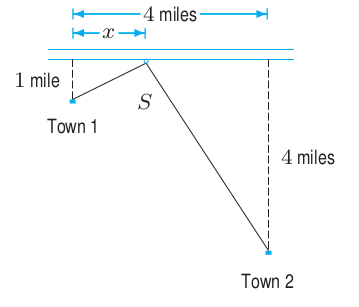
\includegraphics[width=3.7in]{towns.png}
\vspace{-2mm}
%\caption{The amount of energy used by a flying bird.}
\label{fig:towns}
\vspace{-15mm}
\end{center}
\end{figure}

\begin{enumerate}
\setlength{\itemsep}{8mm}

\item Two towns are located near a straight river, as shown in the
  figure above. Town 1 is one mile from the river and town 2 is four
  miles from the river. The two towns both will get drinking water
  from a single pumping station, whose location is indicated by S on
  the figure. There will need to be a pipeline from the pumping
  station to each of the towns. Where should the pumping station be
  located so the length of the pipeline is minimized? 

\newpage
  
\item A bird gathers worms to feed to its young.  To do so, it flies
  from its nest to wherever the worms are, picks up several worms in
  its beak, and then returns to its nest to feed its hungry
  children. A \emph{loading curve}, such as the one shown in
  Fig.~\ref{fig:worms}, shows how the number of worms the bird picks
  up depends on the time the bird spends searching.
  \begin{enumerate}
    \setlength{\itemsep}{1mm}
  \item Why might the shape of the curve be concave down?  
  \item The time it takes the bird to travel from its next to the
    worm-gathering place is represented by the distance PO in
    Fig.~\ref{fig:worms}.  The birds (and its young) want to maximize
    the rate it which it brings worms to the next. This quantity is
    given by:
    \begin{equation}
      \text{Rate Worms Arrive} \, = \, \frac{\text{Number of
          Worms}}{\text{Traveling time} + \text{Searching time}} \;.
    \end{equation}
    \item Draw a line on Fig.~\ref{fig:worms} whose slope is equal to
      the rate at which worms arrive.
    \item Using the figure, estimate the load (number of worms) which
      maximizes the worm arrival rate.
    \item If the traveling time is increased, does the optimal load
      increase or decrease?  Why?
  \end{enumerate}


\begin{figure}[h!]
\begin{center}
\vspace{-1mm}
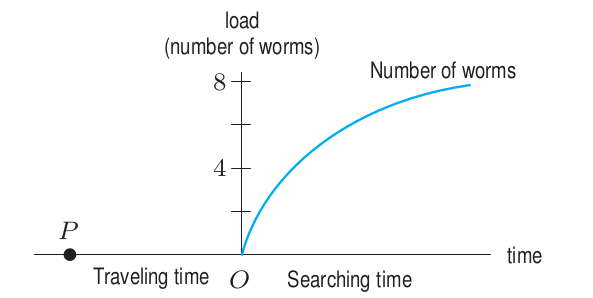
\includegraphics[width=5.60in]{worms.png}
\vspace{-2mm}
\caption{The load curve for the worm-gathering bird.}
\label{fig:worms}
\vspace{-5mm}
\end{center}
\end{figure}

\item The cost of fuel (in dollars per hour) needed to move a boat
  through the water is proportional to the cube of the speed.  (This
  means that $C=kv^3$.)  A ferry boat uses \$100 of fuel per hour if
  it is cruising at 10 km per hour.  The fuel isn't the only cost for
  the ferry. You also need to pay the crew. This cost comes to \$675
  per hour. At what speed should the ferry travel so as to minimize
  the cost per kilometer traveled? 


%\item A ball is thrown straight up from the top of a $30$ meter
%  building. The initial speed of the ball is $v_0$.  The height of the
%  ball as a function of time is given by:
%\begin{equation}
%  y \, = \, -10t^2 + v_0 t + 30 \;.
%\end{equation}
%\begin{enumerate}
%%\setlength{\itemsep}{0mm}
%  \item At what time does the ball reach its highest point?
%  \item What is the maximum height reached by the ball?
%  \item How fast must the ball be thrown so that it makes it $100$
%    meters above the ground?
%\end{enumerate}


\end{enumerate}

\end{document}




  \item Determine an equation for the linear function that generates
    the values in the table below.  

\begin{center}
\begin{tabular}{|| l | l ||}
\hline $x$ & $f(x)$ \\
\hline
5.2 & 27.8 \\
5.3 & 29.2 \\
5.4 & 30.6 \\
5.5 & 32.0 \\
5.6 & 33.4 \\
\hline
\end{tabular}
\end{center}





\end{document}
